 \begin{center}\begin{large} Homework Problems 5
 \end{large}\end{center}
 \bigskip


\begin{problem}
    Calculate $\displaystyle \int f(x)\, dx$:
    \begin{enumerate}
        \item[a) ] $f(x)=3x^2$,
        \item[b) ] $f(x)=x+6\cos x$,
        \item[c) ] $f(x)=\dfrac{3}{x}-1$,
        \item[d) ] $f(x)=\dfrac{4x}{1-2x^2}$,
        % \item[e) ] $f(x)=\dfrac{2x}{1-x^2}$,
        \item[e) ] $f(x)=\text{tg}\,x$.
    \end{enumerate}
\end{problem}


% \bigskip

\begin{problem}%[\textbf{optional, not graded}]
Match the graphs 1-4 to functions i-iv: 
\\~\\
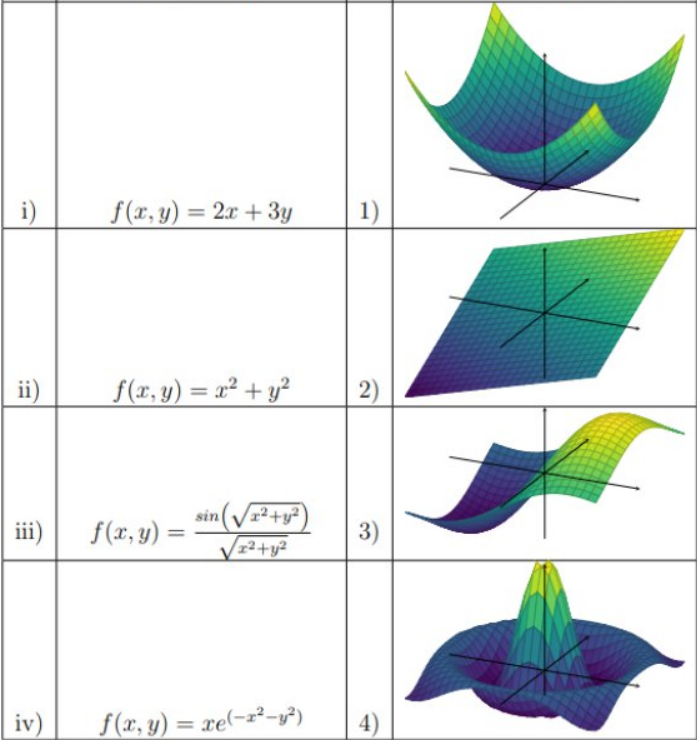
\includegraphics[width=0.6\linewidth]{figs/f(x,y) functions.png}
\\~\\
\end{problem}

% \bigskip

\begin{problem}
Calculate the partial derivatives and Hessian matrices:
\begin{enumerate}
        \item[a) ] $f(x,y)=3x-2y^2$,
        \item[b) ] $f(x,y)=y^7-2x^3+x^2$,
        \item[c) ] $f(x,y)=\sin{xy}$,
        \item[d) ] $f(x,y)=x^y+\dfrac{x}{y}$.
    \end{enumerate}
\end{problem}
\bigskip
\begin{problem}
Calculate the directional derivative:
\begin{enumerate}
        \item[a) ] $f(x, y) = (x-y)^2$ at the point $(1, 2)$ in the direction of $\dfrac{\vv}{\|\vv\|},\,\vv = (3,-4)$,
        \item[b) ] $f(x, y) = x \log y + (1-x) \log (1-y)$ at the point $(\pi, 0)$ in the direction of $\dfrac{\vv}{\|\vv\|},\,\vv = (1,1)$.
    \end{enumerate}

{\small Note: $\log x=\ln x$.}
    
\end{problem}

\bigskip


\begin{problem}
Suppose we roll two fair dice. What is the probability of getting
\begin{enumerate}
    \item[a) ] $2$ on each of them,
    \item[b) ] at least one $1$,
    \item[c) ] exactly one $1$,
    \item[d) ] one $1$ and one $4$,
    \item[e) ] $1$ on the first one and $4$ on the second one?
\end{enumerate}
\end{problem}
\bigskip

\begin{problem}
There are $2$ red, $5$ blue and $6$ yellow pencils in the box. We take two of them out randomly. What is the probability that both of them are
\begin{enumerate}
    \item[a) ] red,
    \item[b) ] of the same color,
    \item[c) ] of different colors,
    \item[d) ] not yellow,
    \item[e) ] not green.
\end{enumerate}
\end{problem}
% \bigskip

\bigskip

\begin{problem}
     \\~\\
\begin{center}
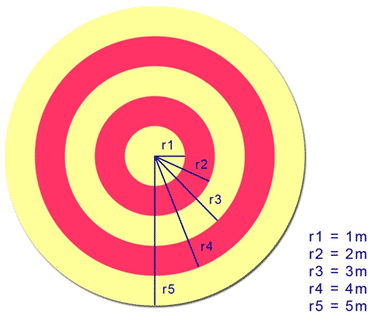
\includegraphics[width=0.5\linewidth]{figs/prob1.png}
\end{center}
\\~\\
Assume that any thrown dart will land somewhere within the circular area. The radius of circle $1$ (the inner-most yellow circle) is $1$ meter. Each radius thereafter increases by $1$ m, as shown. We throw a dart randomly. Find the probability that it lands on
\begin{enumerate}
    \item[a) ] circle $1$,
    \item[b) ] a red circle,
    \item[c) ] a yellow circle.
    
\end{enumerate}
\end{problem}